\subsection{Modificación de la Variable Objetivo}

Con el objetivo de modificar las variancias de las variables objetivo y, intentar adquirir mejores resultados, se ha creído que operar con el valor de la diferencia de las variables objetivos podría ayudar a los modelos a obtener un mejor resultado. Al calcular la variable resultado mediante la resta de las variables home\_team\_score y away\_team\_score, podemos afirmar que un valor positivo en la variable resultado equivale a decir que el equipo local ha salido victorioso del partido, por otra parte, un resultado negativo equivale a la victoria del equipo visitante. Por último, un resultado equivalente a cero, significa empate en el partido. Este estudio ha empezado analizando la matriz de correlación, que se encuentra en la Figura \ref{Conjunto-Datos-Matriz-Correlaciones-Una-Variable}

\begin{figure}[H]
\centering
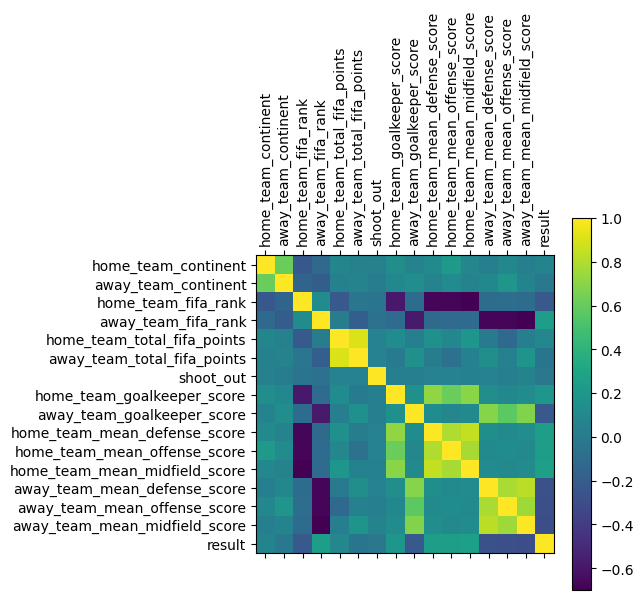
\includegraphics[width=\figsize]{images/correlationMatrixOneObjectiveVariable.png}
\caption{Matriz de correlaciones del conjunto de datos con una variable objetivo}
\label{Conjunto-Datos-Matriz-Correlaciones-Una-Variable}
\end{figure}

Aparentemente, las correlaciones de las variables no se han modificado demasiado, aunque para obtener unos resultados exhaustivos se compararan las Figuras \ref{Conjunto-Datos-Home-Correlaciones}, \ref{Conjunto-Datos-Away-Correlaciones} y \ref{Conjunto-Datos-Resultado-Correlaciones}.

\begin{figure}[H]
\centering
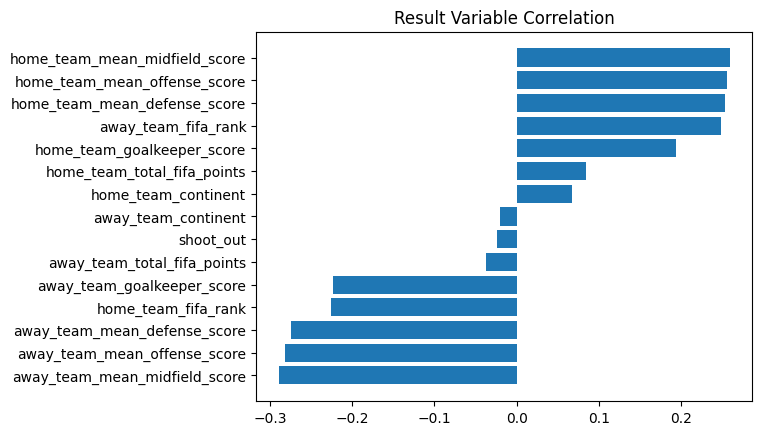
\includegraphics[width=\smallSize]{images/resultCorrelation.png}
\caption{Correlaciones de la variable resultado}
\label{Conjunto-Datos-Resultado-Correlaciones}
\end{figure}

De la gráfica anterior se puede ver la existencia de una correlación positiva entre la variable resultado y todos los datos relacionados con el equipo local. Esta correlación se puede dar a raíz de que una victoria del equipo local equivale a un resultado positivo. Por otra parte, se puede ver como el intervalo de valores de las correlaciones se ha mantenido en relación a las correlaciones del conjunto de datos con dos variables objetivo.